\section{Design}
In this section, we describe the design of \tool{} by focusing on
how our design solves the three challenges discussed in the previous
section.

\subsection{Trace Logging}
The trace information can be logged via some emulators (e.g., QEMU) or 
dynamic binary instrumentation tools (DBI). 
We run a program with the concrete input under the DBI to record the
execution trace.
The trace data has the following information:
\begin{itemize}
    \item Each instruction mnemonics and its memory address.
    \item The operands of each instruction and their concrete values during the 
          runtime.
    \item The value of eflags register. 
    \item The memory address and the length of the sensitive information.
     Most software developers stores sensitive information in an array,
     a variable or a buffer, which means that those data is stored in a contiguous 
     area in the memory. We use the symbol information in the binary to track the 
     address in the memory.
\end{itemize}

\subsection{Instruction Level Symbolic Execution}
\label{InstructionSE}
The main purpose of the step is to generate 
constraints of the input sensitive information from the execution trace. 
If we give the target program a new input which 
is different from the origin input that was used 
to generate the execution trace but still satisfies those constraints,
the new execution trace still have the same control flow and 
data access patterns. 

The tool runs the symbolic execution on the top of the execution traces.
At the beginning of the symbolic execution, the tool creates fresh 
symbols for each byte in the sensitive buffer. For other data in the 
register or memory at the beginning, we use concrete values from the 
runtime information collected in
the previous step. During the symbolic execution for each instruction, 
the tool updates every variable in the memory and registers with a
math formula. The formula is made up with concrete values and 
the input key as the symbols accumulated through the symbolic execution.
For each formula, the tool will check weather it can be reduced
into a concrete values (e.g., $k_1+12-k_1 = 12$ ). 
If so, the tool will only use the concrete values in the 
following symbolic execution.

\subsubsection{Verification and Optimization}
We run the symbolic execution(SE) on the top of x86 instructions.
In other words, we don’t rely on any intermediate languages to 
simplify the implemetation of symbolic execution. 
While the implementation itself 
has a lot of benefits (Better performance, accurate memory model), 
we need to implement the symbolic execution 
rules for each X86 instruction. 
However, due to the complexity of X86, it is inevitable to make mistakes. 
Therefore, we verify the correctness of the SE engine during the execution. 
The tool will collect the runtime information (Register values, 
memory values) and compare them with the formula generated from the 
symbolic execution. Whenever the tool finishes the symbolic execution 
of each instruction, the tool will compare the formula for each symbol 
and its actual value. If the two values don't match, we check the code
and fix the error. Also, if the formula doesn't contain any symbols,
the tool will use the concrete value instead of symbolic execution.

\subsubsection{Secret-dependent control-flows}
An adversary can infer sensitive information from secret dependent control-flows. 
There are two kinds of control-transfer instructions: the unconditional 
control-transfer instructions and the conditional transfer instructions.
The unconditional instructions, like CALL, JUMP, RET transfer control
from one code segment location to another. Since the transfer is 
independent from the input sensitive information, an attacker was 
not able to infer any sensitive information from the control-flow. 
So the unconditional control-transfer doesn't leak any information 
based on our threat model. During the symbolic execution, 
we just update the register information and memory cells with 
new formulas accordingly.

The conditional control-flow transfer instructions, like conditional jumps,
depending on CPU states, may or may not transfer control flows.
For conditional jumps, the CPU will test if certain condition flag 
(e.g., CF = 0, ZF =1) is met and jump to the certain branches respectively.
The symbolic engine will compute the flag and represent the flag 
in a symbol formula. Because we are running on a symbolic execution 
on a execution trace, we know which branch is executed.
If a conditional jump uses the CPU status flag, we will generate 
the constraint accordingly.

\begin{figure}[ht]
      \centering
      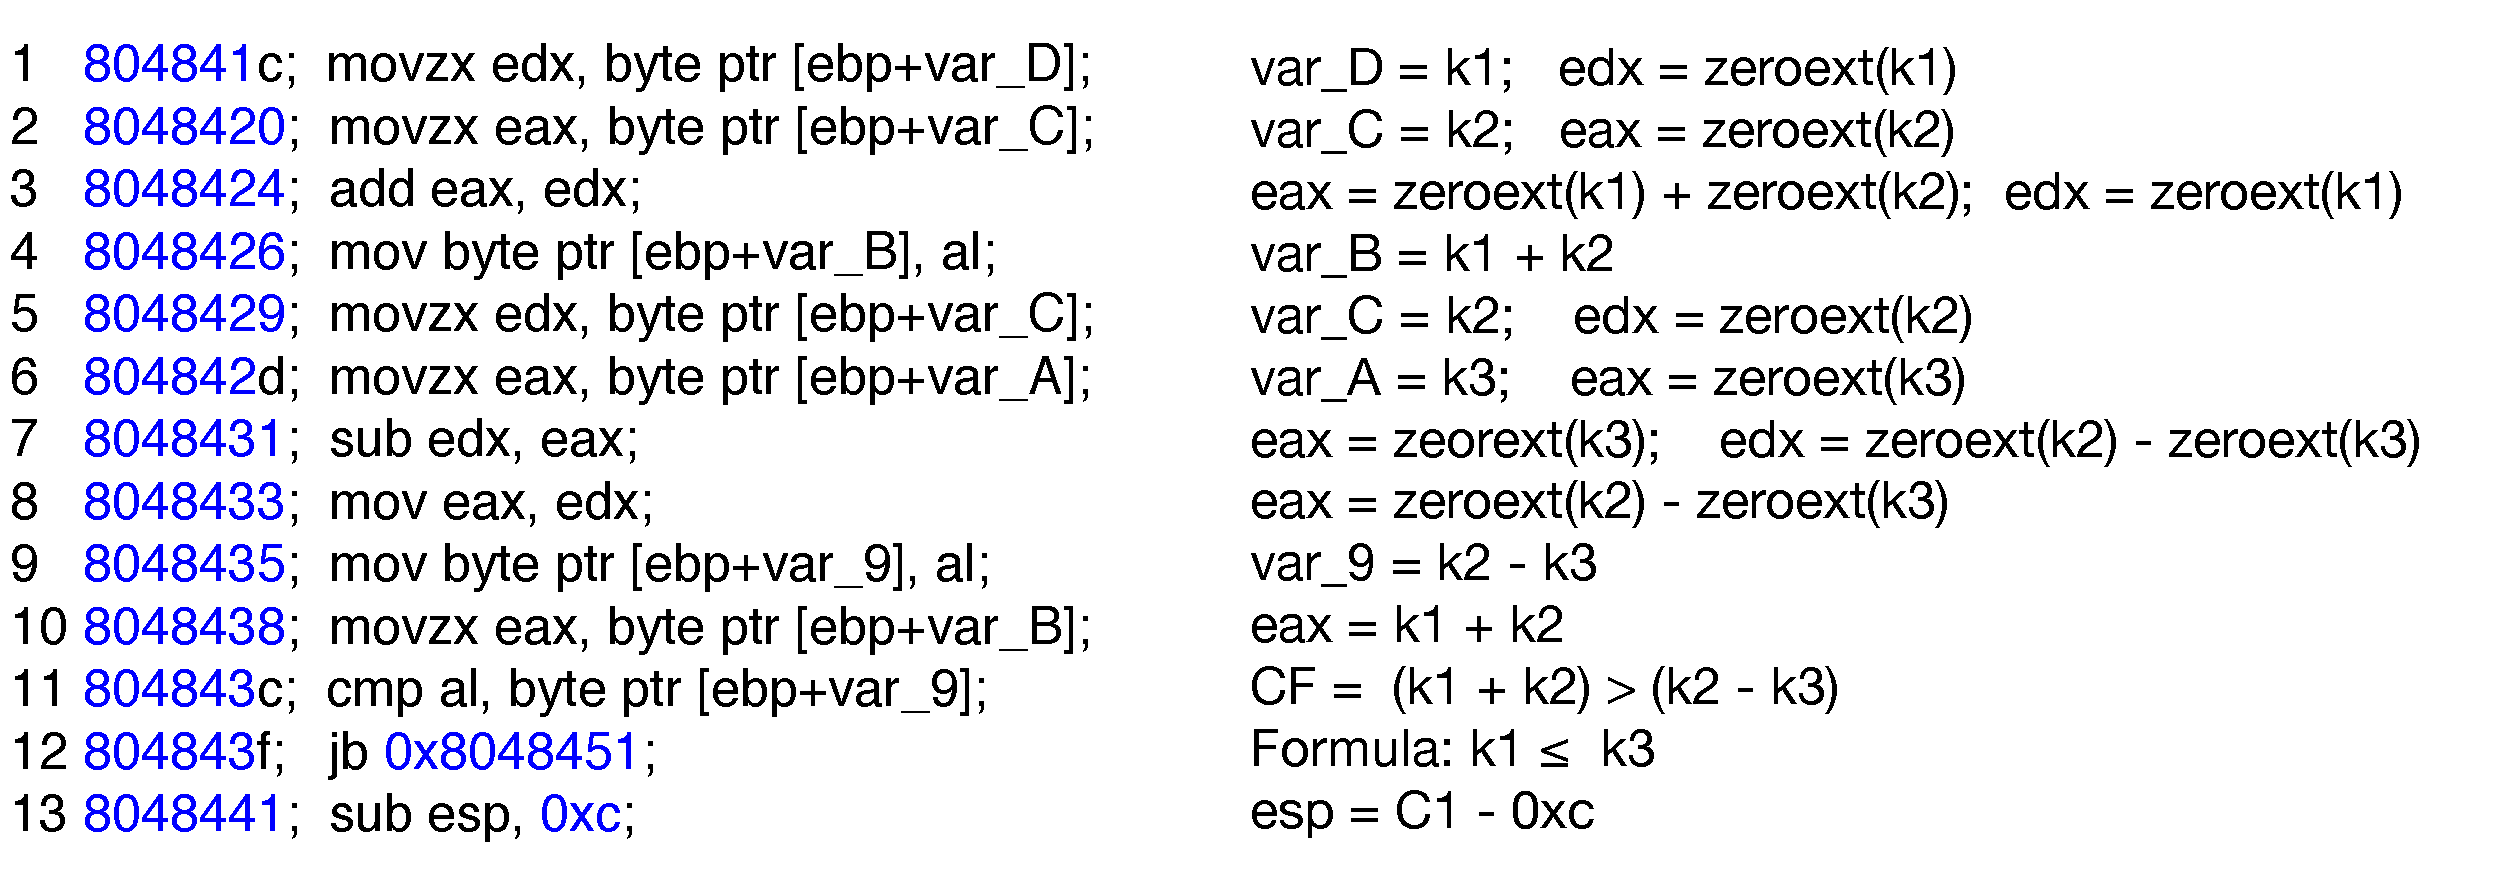
\includegraphics[width=\columnwidth]{./figures/secretCF.pdf}
      \caption{The workflow of \tool{}}
      \label{fig:Test}
  \end{figure}

For examples,

\begin{lstlisting}
...
0x0000e781      add dword [local_14h], 1
0x0000e785      cmp dword [local_14h], 4
0x0000e789      jne 0xe7df
0x0000e78b      mov dword [local_14h], 0
...
\end{lstlisting}

At the beginning of the instruction segment, the value at the 
address of local14h can be written as $F(\vec{K})$. At the address e785, 
the value will be updated with $F(\vec{K})+1$. Then the code compares 
the value with 4 and use the result as a conditional jump. 
Based on the result, we can have the following formula:

$$F(\vec{K}) + 1 = 4$$

The formula, together with the memory address (0xe789) is store
as a \textit{formula tuple (address, formula)}. 
Each formula tuple represents one leakage site.

\subsubsection{Secret-dependent data access}
Like input-dependent control-flow transfers, an adversary can also infer 
sensitive information from the data access pattern as well. 
We try to find this kind of leakages by checking 
every memory operand of the instruction. We generate the memory addressing 
formulas. As discussed before, every symbols in the formula is the input key. 
If the formula doesn’t contain any symbols, the memory access is independent 
from the input sensitive information and won’t leak any sensitive information 
according to our threat model. Otherwise, we will generate the constraint for
the memory addressing. We model the memory address with a symbolic formula 
$F(\vec{K})$. 
Because we also have the concrete value of the memory address $Addr1$. 
Inspired by the work from~\cite{203878}, the formula can be written as:

$$F(\vec{K}) >> L = Addr1 >> L$$

The $L$ represents the minimum memory address granularity that an attacker 
can observe. For example, Flush and Reload can distinguish between different
cache lines, which means the value of L is 6.

\subsection{Information Leakage Estimation}

In this section, we present the alogorithm to calculate the information
leakage with the definition~\ref{def}. 

\subsubsection{Problem Statement}
From the above step~\ref{InstructionSE}, we can generate the constraint 
for each unique leakage site on the execution trace.
The only variables in those constraints are the sensitive data represented
with $k_1, k_2, ... , k_n$. Suppose the address of the leakage site is $i$,
we use $C_i$ to denote the constraint. For mutiple leakage sites, 
as each leakage site has one constraint, we can 
use the conjunction of those constraints to represent those leakage sites. 

According to the definition~\ref{def}, to calculate the amount of leaked 
information, the key is to calculate $\frac{|K|}{|K^o|}$. $|K^o|$ represent
the set that contain every input keys that satisfy the constraint. As the 
cardinality of $K$ is known, the key problem is to know the cardinality of
$K^o$. Suppose an attacker can observe $n$ leakage sites, and each leakage site has
the following constraints: $C_1, C_2, ..., C_n$ respectively. 
The total leakage has the constraint $F_{c1c2...cn} = C_1 \land C_2 \land C_3
\land ... \land C_n$. The problem of estimating the total leaked information 
can be transfered into counting the number of different solutions that satisfies
the constraint $F_{c1c2...cn}$. 

A native method for approximating 
the result is to pick $k$ elements from $K$ and check how many of them are also
contained in $K^o$. If $q$ elements are also in $K^o$. In expectation, we can
use $\frac{k}{q}$ to approximate the value of $\frac{|K|}{|K^o|}$.

However, as the discussion in ~\ref{MCreasons},
the above sampling method will typically fail due to the following two reasons:

\begin{itemize}
      \item The curse of dimensionality. $F_{c1...cn}$ is the conjunction of many
      constraints. Therefore, the input variables of each constraints will also be 
      the input variables of the $F_(c1...cn)$. The sampling method will fail as 
      $n$ increases. For example, when $n$ equals to 2, the whole serach space is 
      a $256^2$ cube. If we want to the distance between each points equals to 1,
      we need $256^2$ points. When $n$ equals to 10, we need $256^8$ points if we 
      still we want the distance between each points equals to 1. As a result, the 
      error of the result based on sampling method will increases exponentially with
      adding dimension. 

      \item The number of satisfying solution could be exponentially small.
      According to Chernoff bound, we need to exponentially many samples to get 
      a tight bound. On an extreme situation, if the constraint only has one unique
      satisfying solutions. 
\end{itemize}

\subsubsection{Definitions}
We apply two preprocessing steps before running the Monte Carlo sampling. First,
we try to simplify those formulas by applying some normalizations rules. After
that, we split those formulas into multiple groups.

The goal of the normalization is to simplify the formulas. 
Each formulas will be evaluated multiple times with different input 
during the following sampling, 
we would like to make those formula simpler to reduce the whole execution time.  
Each formula is implemented as a abstract syntax tree. We apply a series of 
normalization rules (e.g. key1 xor key1 = 0) to simplify the formula.

After that, we split the formula tuple into multiple groups. 
Each group consists of different formulas but with the same memory address.
In other words, those formulas in the same group represent one leakage
site. The instructions inside a loop are executed multiple times with
the different item from the input buffer. We group them together to 
know the total information leakage.

The only symbol in the original formula is the key. 
An adversary who wants to infer the sensitive data based on side-channel 
attacks can't observe the sensitive information directly. 

\subsubsection{Motivation}
The adversary, however, can observe the memory access pattern of the software. 
If the attacker can observe one leakage site, the attack is modeled as one formula. 
If he observes mutiple information leakage, the attack is modeled as the conjoint 
of those formulas. Calculating the total information leakage can be reduced to the
problem of approximating the number of solutions. This is a \#P problem.

One intuition way is to use the Monte Carlo method. However, 
as the discussion in the previous section~\ref{MCreasons},
the number of satisfying keys could be exponentially small. Imagine an attacker 
who can recover one unique key after the attack, in such case, 
the conjoint of formula F = (f(k)) only has one solution.
Also, the target program may have mutiple inputs. When the number of input
symbols arises, the simple Monte Carlo may suffer from the curse of dimensionality,
which means the accuracy of the result drops dramatically when the
number of input symbols increases. 

We adopt the Markov Chain Monte Carlo (MCMC) to estimate the number of 
satisfying solutions. The basic idea is to construct a Markov Chain that
has the desired distribution.

\textit{Definition:}
Starting from here, we present the formal definition of the MCMC algorithm.
First, we introduce the definition of the concept of the algorithm.


\newtheorem{theorem}{Theorem}[section]

\begin{theorem}
      If $F={A_1,A_2,...,A_n}$ is a finite collection of closed sets then 
      $\cup_{i}^{n}A_i$ is a closed set.
\end{theorem}

\subsubsection{MCMC Algorithm}
In the section, we present the detail of MCMC algorithm for counting the 
cardinality of $K^o$. We will fisrt present the description of the 
MCMC and then explain the algorithm with a concrete example.
\begin{enumerate}
      \item Start with the concrete input $\vec{k} = (k_0, k_1, k_2, ..., k_n)$,
      $\vec{k}$ should be the on valid solution which satisfies the constraint
      $F = C_1(\vec{k})\land C_2(\vec{k})\land C_2(\vec{k}) \land ... \land C_m(\vec{k})$
      \item for t = 1, 2, 3,..., N
\end{enumerate}